\chapter{Theoretical Framework}

\label{Chapter3}

\section{Causal Setup and the Markdown DAG}
\label{sec:causal-setup-dag}

The pricing question is causal rather than purely predictive: what would happen to weekly sales if the same reference-week were assigned a different price? Historical associations cannot answer this directly because markdowns are not randomized. Products with weak momentum or high remaining stock are more likely to receive deeper discounts, so discount and sales can be negatively associated even when the causal effect of a discount on demand is positive.

In causal inference, this setup can be described through three main concepts: treatment, outcome, and confounders. The treatment is the decision or variable whose effect is being studied, the outcome is the result being measured, and confounders are background variables that influence both the treatment and the outcome. Without controlling for these confounders, the estimated relationship between price and sales may confuse the true customer demand response with background factors such as product timing, stock pressure, or prior sales momentum.

A Directed Acyclic Graph (DAG) makes this structure explicit \cite{pearl2009causality}. Using the variables introduced in Chapter~\ref{Chapter2}, the treatment is discounted price, the selling price after markdown, and the outcome is weekly units sold. The confounders are the pre-pricing context variables described in Section~\ref{sec:variables-modelling}. These variables capture calendar timing, product characteristics, original price, stock pressure, sales momentum, and material composition before the markdown decision is made.

\begin{figure}[ht]
    \centering
    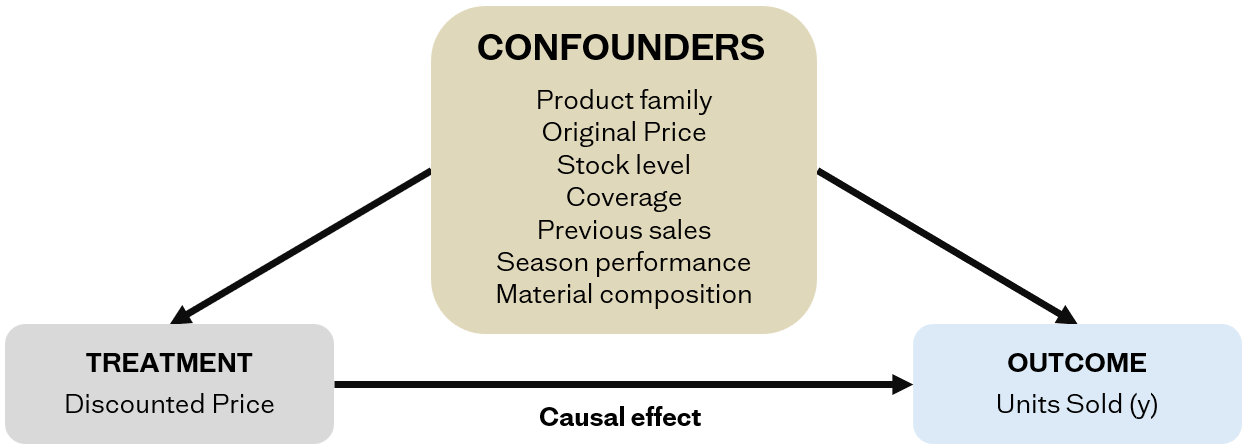
\includegraphics[width=0.95\textwidth]{Figures/dag.png}
    \caption{Simplified DAG for the markdown pricing causal setup.}
    \label{fig:markdown-dag}
\end{figure}

Figure~\ref{fig:markdown-dag} summarizes the main identifying assumption: the confounders can affect both the assigned price and future sales, while the causal effect of interest runs from the price decision to weekly demand. No variables observed after the price is set are included, as this would distort the estimated causal effect. This clear separation motivates the use of the Double Machine Learning (DML) method explained in the next sections.


\section{Potential Outcomes and Double Machine Learning}
\label{sec:potential-outcomes-dml}

The potential outcomes framework defines $Y(t)$ as the weekly sales that would be observed if a reference-week were assigned treatment level $t$ \cite{rubin1974causal,imbens2015causal}. Only one potential outcome is observed for each reference-week, so identification requires unconfoundedness: conditional on $X$, the remaining variation in price is treated as if it were random for estimating demand response \cite{angrist2009mostlyharmless}. In the continuous-treatment specification used in this thesis, the causal effect is represented by a marginal parameter, $\theta$, which approximates the expected change in demand caused by a one-unit change in price. Double Machine Learning (DML) implements this adjustment with flexible nuisance models while targeting this causal parameter \cite{chernozhukov2018dml}. The partially linear model is

\begin{equation}
Y = \theta T + g(X) + \varepsilon,
\label{eq:plr-model}
\end{equation}

where $Y$ is sales, $T$ is price, $g(X)$ captures the structural non-linear effect of context, and $\theta$ is the average marginal causal effect.

To isolate $\theta$ without relying on strict parametric assumptions, DML separates the estimation of the background context from the causal relationship itself. Let $l(X)=\mathbb{E}[Y\mid X]$ represent the expected demand given the commercial context, and let $m(X)=\mathbb{E}[T\mid X]$ represent the expected price dictated by historical pricing rules. These nuisance functions are used to remove the explainable components from both variables. Specifically, the DML algorithm proceeds in three steps for each observation $i$:

\begin{enumerate}
    \item \textbf{Residualize the outcome}: Estimate the expected demand, $\hat{l}(X_i)$, and compute the demand residual:
    \begin{equation}
    \tilde{Y}_i = Y_i - \hat{l}(X_i).
    \end{equation}
    \item \textbf{Residualize the treatment}: Estimate the expected price, $\hat{m}(X_i)$, and compute the price residual:
    \begin{equation}
    \tilde{T}_i = T_i - \hat{m}(X_i).
    \end{equation}
    \item \textbf{Estimate the causal effect}: Regress the demand residuals $\tilde{Y}_i$ on the price residuals $\tilde{T}_i$ to obtain the causal estimate $\hat{\theta}$.
\end{enumerate}

The intuition behind this process is to ask what remains after the usual business context has been stripped away. In the first step, LightGBM predicts demand using only the background variables $X$. Subtracting this prediction gives the demand residual, $\tilde{Y}_i$, which represents the portion of sales not explained by stock, timing, product characteristics, or past performance. In the second step, the same logic is applied to price. The price residual, $\tilde{T}_i$, captures the portion of the assigned price that deviates from the historical markdown policy. Regressing $\tilde{Y}_i$ on $\tilde{T}_i$ then measures how these two unexplained components move together, isolating the price effect from the confounding influence of the pre-pricing context.

In this thesis, the nuisance models are estimated with LightGBM and cross-fitting is done by season to prevent temporal leakage. Crucially, the resulting orthogonal score structure of DML makes the final estimate less sensitive to first-order approximation errors in the machine learning nuisance models, which permits flexible machine learning in the first two stages while still targeting a causal parameter \cite{chernozhukov2018dml}.

\section{From ATE to CATE with Causal Forests}
\label{sec:cate-causal-forests}

A single Average Treatment Effect is useful for diagnosis but too general for markdown decisions. Price response can vary by product family, sale week, stock level, original price, and recent momentum, while the optimizer needs one curve per reference-week. The target is therefore the Conditional Average Treatment Effect (CATE), which allows the effect to vary with the covariates of each reference-week.

In the continuous-treatment setting used in this thesis, the heterogeneous effect is interpreted as a local one-euro price effect. For a reference-week with covariates $X=x$, the CATE can be written as

\begin{equation}
\tau(x)=\mathbb{E}[Y(t+1)-Y(t)\mid X=x].
\end{equation}

Here, $t$ represents discounted price. Therefore, $\tau(x)$ measures the expected change in the outcome when discounted price increases by one euro for reference-weeks with characteristics $X=x$. While the ATE summarizes one average price effect for the whole sample, the CATE allows this effect to vary across reference-weeks.

In the final specification of this thesis, $Y$ is the logarithm of season-normalized weekly units sold and $T$ is discounted price. Therefore, the estimated $\tau(x)$ is interpreted as a local semi-elasticity: $100\times\tau(x)$ is the approximate percentage change in normalized weekly units sold associated with a one-euro increase in discounted price for a reference-week with covariates $X=x$.

After DML residualization, the heterogeneous final stage can be written as

\begin{equation}
\tilde{Y}_i=\tau(X_i)\tilde{T}_i+\eta_i,
\end{equation}

where $\tilde{Y}_i=Y_i-\hat{l}(X_i)$ and $\tilde{T}_i=T_i-\hat{m}(X_i)$. Instead of estimating a single global slope, the Causal Forest estimates how this residualized price effect varies across the covariate space.

Causal Forests estimate $\tau(X_i)$ by growing trees that split observations to separate treatment effects rather than to improve outcome prediction \cite{wager2018hteforest,athey2019causalforests,athey2019grf}. The forest relies on honest trees: one subsample determines how the trees are split, while a separate subsample estimates the treatment effects inside the resulting leaves. This partition reduces adaptive overfitting and makes local CATE estimates more stable.

In this thesis, Causal Forests move the model from a global ATE to reference-week-level treatment effects. The DML residualization is performed explicitly with LightGBM nuisance models, and the resulting residuals are passed to EconML's \texttt{CausalForest}, which is used as the heterogeneous final stage of the pipeline \cite{battocchi2019econml,oprescu2019orf,syrgkanis2021econml}.

\section{From Local Effects to Markdown Curves}
\label{sec:local-effects-markdown-curves}

The Causal Forest outputs one local price effect $\hat{\tau}(X_i)$ for each reference-week $i$. This is not yet a full markdown curve. To build the curve, each possible discount is first converted into its implied discounted price:

\begin{equation}
P_i(d)=P_i^{0}(1-d).
\end{equation}

The curves are normalized at the reference discount $d_0=0.20$. Since the model is log-linear, the predicted sales multiplier at discount $d$ is

\begin{equation}
\widehat{m}_i(d)=
\exp\left(\hat{\tau}(X_i)\left[P_i(d)-P_i(d_0)\right]\right).
\end{equation}

This gives the expected demand at discount $d$ relative to the demand at the 20\% reference discount. If $\hat{\tau}(X_i)$ is negative, deeper discounts imply lower discounted prices and therefore higher predicted sales.

To evaluate revenue, the sales multiplier is adjusted by the relative discounted price:

\begin{equation}
\widehat{r}_i(d)=
\widehat{m}_i(d)\frac{P_i(d)}{P_i(d_0)}
=
\widehat{m}_i(d)\frac{1-d}{1-d_0}.
\end{equation}

The break-even sales multiplier is

\begin{equation}
m_i^{BE}(d)=
\frac{P_i(d_0)}{P_i(d)}
=
\frac{1-d_0}{1-d}.
\end{equation}

A discount improves revenue relative to the 20\% reference point when the predicted sales multiplier is above this break-even curve. This is how the local Causal Forest effects are converted into the markdown curves evaluated in the results.
